\documentclass[11pt,a4paper]{report}
\usepackage[spanish,es-nodecimaldot]{babel}	% Utilizar español
\usepackage[utf8]{inputenc}					% Caracteres UTF-8
\usepackage{graphicx}						% Imagenes
\usepackage[hidelinks]{hyperref}			% Poner enlaces sin marcarlos en rojo
\usepackage{fancyhdr}						% Modificar encabezados y pies de pagina
\usepackage{float}							% Insertar figuras
\usepackage[textwidth=390pt]{geometry}		% Anchura de la pagina
\usepackage[nottoc]{tocbibind}				% Referencias (no incluir num pagina indice en Indice)
\usepackage{enumitem}						% Permitir enumerate con distintos simbolos
\usepackage[T1]{fontenc}					% Usar textsc en sections
\usepackage{amsmath}						% Símbolos matemáticos

% Comando para poner el nombre de la asignatura
\newcommand{\asignatura}{Simulación de Sistemas}
\newcommand{\autor}{José María Sánchez Guerrero}
\newcommand{\titulo}{Práctica 1}
\newcommand{\subtitulo}{Diferentes Modelos de Simulación}

% Configuracion de encabezados y pies de pagina
\pagestyle{fancy}
\lhead{\autor{}}
\rhead{\asignatura{}}
\lfoot{Grado en Ingeniería Informática}
\cfoot{}
\rfoot{\thepage}
\renewcommand{\headrulewidth}{0.4pt}		% Linea cabeza de pagina
\renewcommand{\footrulewidth}{0.4pt}		% Linea pie de pagina

\begin{document}
\pagenumbering{gobble}

% Pagina de titulo
\begin{titlepage}

\begin{minipage}{\textwidth}

\centering

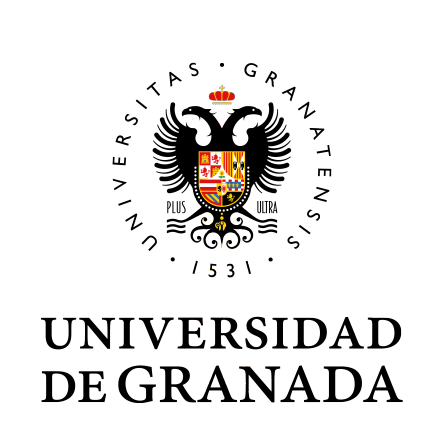
\includegraphics[scale=0.5]{img/ugr.png}\\

\textsc{\Large \asignatura{}\\[0.2cm]}
\textsc{GRADO EN INGENIERÍA INFORMÁTICA}\\[1cm]

\noindent\rule[-1ex]{\textwidth}{1pt}\\[1.5ex]
\textsc{{\Huge \titulo\\[0.5ex]}}
\textsc{{\Large \subtitulo\\}}
\noindent\rule[-1ex]{\textwidth}{2pt}\\[3.5ex]

\end{minipage}

\vspace{0.5cm}

\begin{minipage}{\textwidth}

\centering

\textbf{Autor}\\ {\autor{}}\\[2.5ex]
\textbf{Rama}\\ {Computación y Sistemas Inteligentes}\\[2.5ex]
\vspace{0.3cm}


\includegraphics[scale=0.3]{img/etsiit.jpeg}

\vspace{0.7cm}
\textsc{Escuela Técnica Superior de Ingenierías Informática y de Telecomunicación}\\
\vspace{1cm}
\textsc{Curso 2018-2019}
\end{minipage}
\end{titlepage}

\pagenumbering{arabic}
\tableofcontents
\thispagestyle{empty}				% No usar estilo en la pagina de indice

\newpage

\setlength{\parskip}{1em}

\chapter{Mi primer modelo de simulación de MonteCarlo}

Este modelo de simulación lo vamos a tratar con el problema del \textit{aparcamiento}, en el cual un coche se dispone
a aparcar a una distancia $x$ de su destino. También dispondremos de variables como el número de plazas que alcanza a
ver el conductor desde su posición o la probabilidad de que esa plaza esté ocupada o no. El ejercicio consiste en elegir
una plaza de aparcamiento $c$ en la cual el conductor, ni se quede muy corto ni se pase, es decir, que encuentre un
valor que minimice la distancia esperada desde el lugar de aparcamiento hasta el objetivo.


\section{Experimentación inicial}

Para hacernos una idea de los valores que obtendremos y los parámetros que más afectan al rendimiento de este modelo,
vamos a realizar una ejecución inicial del programa con todos los valores que trae por defecto.

Estos parámetros y sus valores son los siguientes:

\begin{itemize}
	\item Número de veces que se repite para hacer la media: 100000
	\item Posición de destino $x$: 100
	\item Número de posiciones siguientes que podemos ver: 2
	\item Probabilidad de que el aparcamiento esté ocupado: 0.9 (90\%)
\end{itemize}

El resultado de la ejecución es el siguiente: la mejor posicion inicial ha sido $c=94$ con una distancia media hasta
el destino de 6.50395 posiciones. Este resultado ya nos da una idea de cuáles van a ser los mejores valores $c$, y es que
cuanto más cerca empecemos a buscar aparcamiento, más se reducirá la distancia hasta el destino.

A continuación, vamos a mostrar una gráfica para poder comprobar esto que acabamos de decir y saber si estamos en lo
cierto o no.

\begin{figure}[H]
\centering
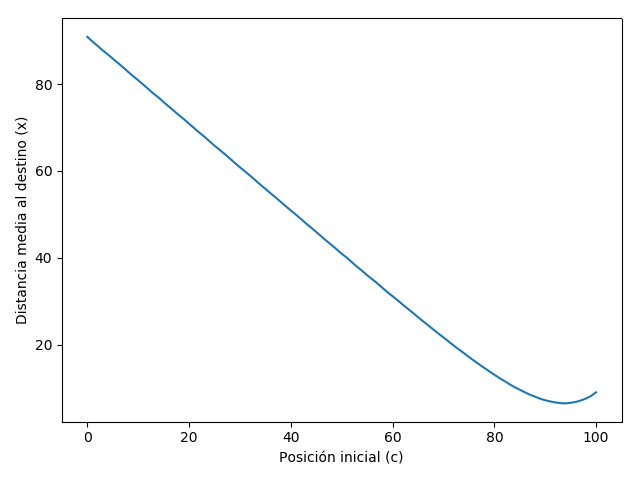
\includegraphics[scale=0.7]{img/x-100-2-90.png}
\caption{Valor medio de la distancia a medida que nos acercamos a $x=100$}
\end{figure}

Como podemos ver en la gráfica, se cumple lo que habíamos mencionado. Esto se debe a que nos quedamos con el primer
sitio que encontramos, y si empezamos a buscar desde una plaza muy alejada del destino, terminaremos aparcando en
una plaza bastante alejada también.

En la gráfica también vemos que a partir de $c=94$ se aumenta la distancia al destino, ya que probablemente no encuentre
ninguna posición cercana al destino y se pase. Esto nos hace pensar que, pese a que el $c=94$ sea la mejor plaza teniendo
en cuenta únicamente la media, puede dar unos resultados muy diferentes, es decir, que puede tener una varianza más alta
respecto a otras posiciones.

Al igual que hemos hecho con la distancia al destino, a continuación vamos a mostrar una gráfica conlos valores que nos
ofrece la desviación típica y los mejores resultados.

\begin{figure}[H]
\centering
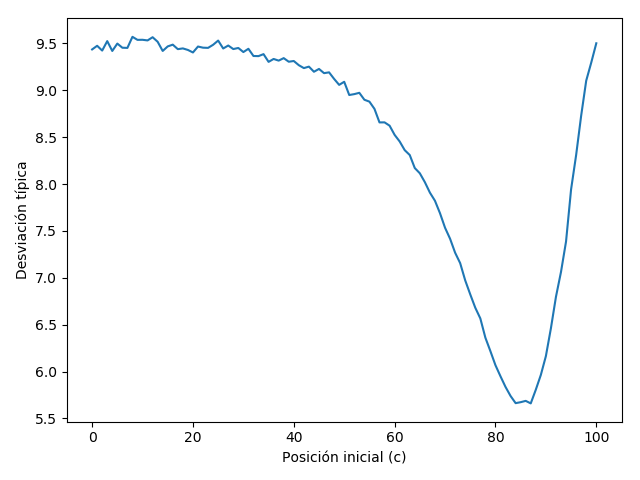
\includegraphics[scale=0.7]{img/dt-100-2-90.png}
\caption{Valor medio de las desviaciones típicas a medida que nos acercamos a $x=100$}
\end{figure}

El resultado de la ejecución es el siguiente: la posicion inicial con menos desviación típica ha sido $c=84$ con un valor
medio de 5.651982. Por lo que podemos ver en la gráfica, para los valores que hay alrededor del $c=94$, que es el que
menor distancia al destino tenía, tiene unos valores de desviación típica más altos. Esto nos confirma que, efectivamente,
empezar a buscar tan cerca del destino nos puede salir en ocasiones muy bien pero en otras no tanto.


\section{Experimentación modificando los parámetros}

En este apartado vamos a ver que sucede cuando modificamos los parámetros de nuestro modelo y cómo afectan al comportamiento
del sistema. 

\subsection{Posición de destino}

Vamos a comenzar modificando la posición de destino, dándole por ejemplo un valor de \textbf{x=50} y otro de \textbf{x=200}.
El resultado de la ejecución es el siguiente.

\newpage

Para \textbf{x=50} el resultado de la ejecución nos dice que la mejor posicion inicial ha sido $c=44$ con una distancia media hasta
el destino de 6.50545 posiciones; y en cuanto a la desviación típica, que la posicion inicial que ha obtenido un valor más
bajo sido $c=35$ con una media de 5.646533.

A continuación, las dos gráfica correspondientes a los resultados:

\begin{figure}[H]
\centering
\begin{minipage}{0.5\textwidth}
  \centering
  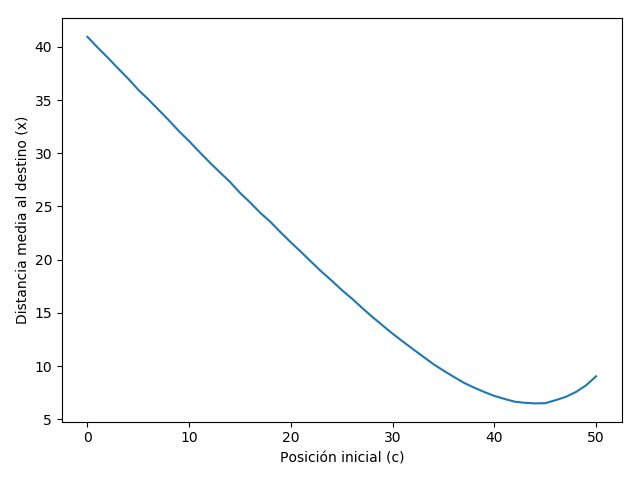
\includegraphics[scale=0.4]{img/x-50-2-90.png}
\end{minipage}%
\begin{minipage}{0.5\textwidth}
  \centering
  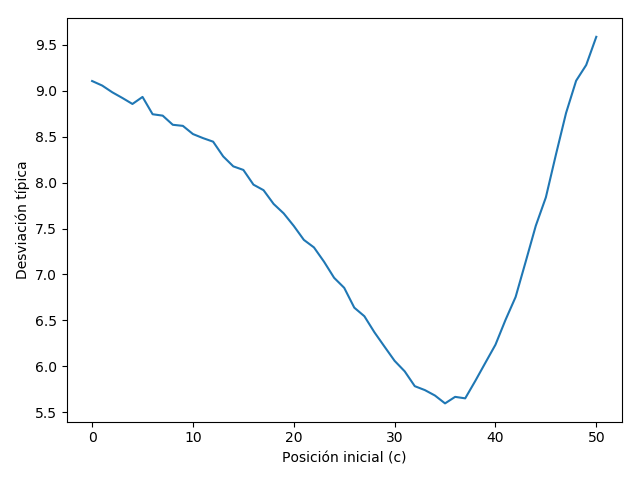
\includegraphics[scale=0.4]{img/dt-50-2-90.png}
\end{minipage}
\caption{Valores medios de las distancias y las desviaciones típicas a medida que nos acercamos a x = 50}
\end{figure}

Podemos ver que la posición $c$ en la que se empieza a buscar aparcamiento lógicamente ha cambiado, ya que no tenemos tantas
plazas como teníamos anteriormente. Sin embargo, observando los valores medios de la distancia y de la desviación típica,
podemos observar como son muy parecidos a los que ya teníamos (incluso el valor de $c$ con la menor desviación típica está
aproximadamente 10 por debajo del que tienen las distancias).

Si nos fijamos en las gráficas, vemos que son muy similares a las que obtuvimos en la primera ejecución, y por tanto, podemos
confirmar que este parámetro no influye demasiado en el modelo.

Vamos a ver ahora que sucede con un \textbf{x=200}. El resultado de la ejecución nos dice que la mejor posicion inicial ha sido
$c=194$ con una distancia media hasta el destino de 6.46297 posiciones; y en cuanto a la desviación típica, que la posicion
inicial que ha obtenido un valor más bajo sido $c=187$ con una media de 5.60064.

\begin{figure}[H]
\centering
\begin{minipage}{0.5\textwidth}
  \centering
  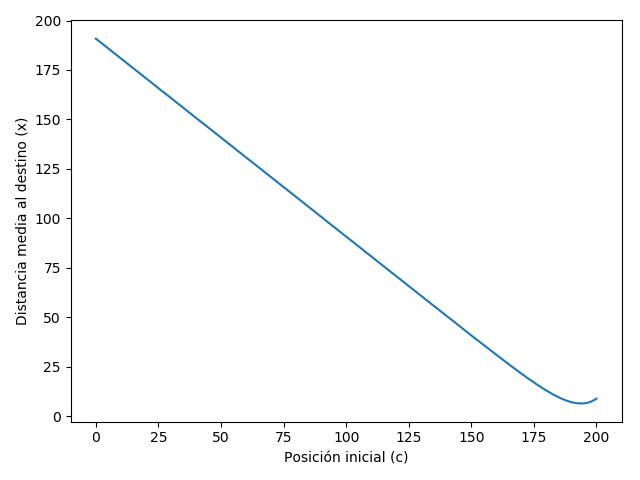
\includegraphics[scale=0.4]{img/x-200-2-90.png}
\end{minipage}%
\begin{minipage}{0.5\textwidth}
  \centering
  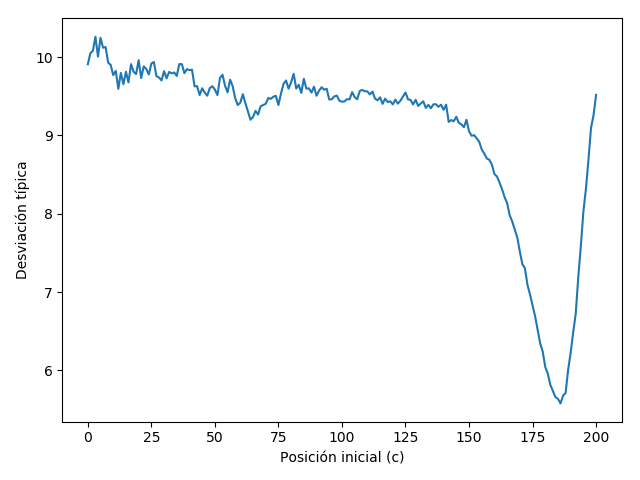
\includegraphics[scale=0.4]{img/dt-200-2-90.png}
\end{minipage}
\caption{Valores medios de las distancias y las desviaciones típicas a medida que nos acercamos a x = 200}
\end{figure}

Al igual que en las otras ejecuciones, tanto los resultados como las gráficas también son muy similiares (los valores cambian
la forma de la curva, pero el patrón que siguen es muy parecido), lo cual nos sirve para asegurar todavía más lo comentado
anteriormente.

\subsection{Número de posiciones vistas}

El siguiente parámetro que vamos a modificar va a ser el número de posiciones que vamos a poder ver desde la que nos encontramos.
Este parámetro tiene por defecto un valor de 2, por lo que vamos a probar por ejemplo con 0 y con 10. El resto de parámetros los
dejaremos como estaban en un principio.

El resultado de las simulaciones con estos parámetros son los siguientes:
\begin{itemize}[label=\textbullet]
	\item Para \textbf{vision=0} la mejor posicion inicial ha sido $c=94$ con una distancia media hasta el destino de 6.54038posiciones;
	y la mejor desviación típica, se ha obtenido en $c=86$ con una media de 5.642444.
	\item Para \textbf{vision=10} la mejor posicion inicial ha sido $c=92$ con una distancia media hasta el destino de 5.65583 posiciones;
	y la mejor desviación típica, se ha obtenido en $c=85$ con una media de 5.448542.
\end{itemize}

En este caso vemos cómo la distancia media hasta el destino se está reduciendo a medida que aumentamos el número de posiciones que
observamos desde el vehículo. No obstante, las desviaciones típicas, pese a que se han reducido un poco, el cambio tampoco es muy grande.

Vamos a mostrar las gráficas de estas dos ejecuciones a ver si podemos ver algo más relevante en ellas.

\begin{figure}[H]
\centering
	\begin{minipage}{0.5\textwidth}
	  \centering
	  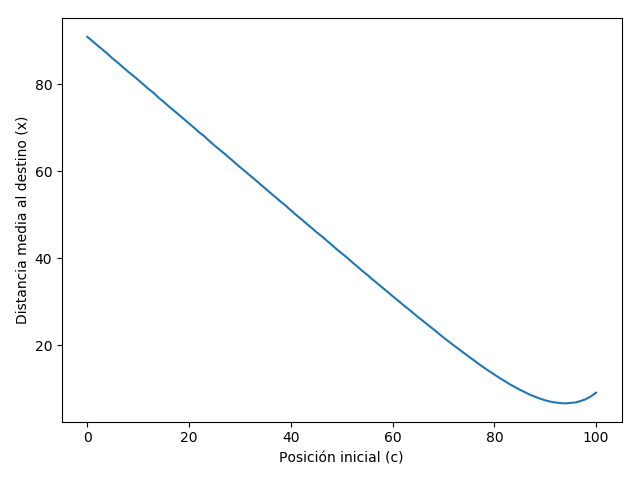
\includegraphics[scale=0.4]{img/x-100-0-90.png}
	\end{minipage}%
	\begin{minipage}{0.5\textwidth}
	  \centering
	  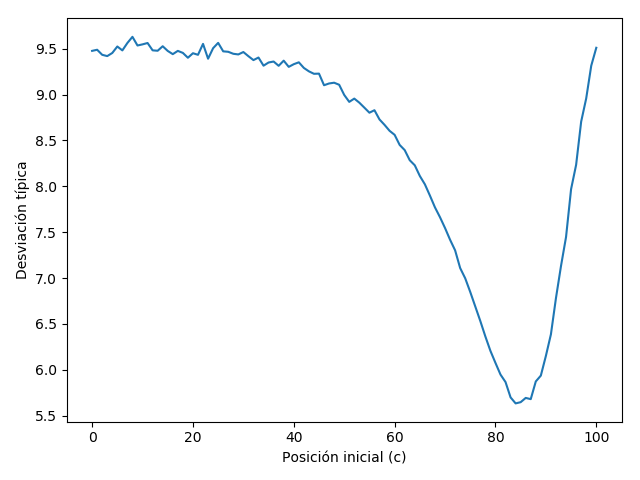
\includegraphics[scale=0.4]{img/dt-100-0-90.png}
	\end{minipage}
\caption{Valores medios de las distancias y las desviaciones típicas con visión=0}
\end{figure}

\begin{figure}[H]
	\begin{minipage}{0.5\textwidth}
	  \centering
	  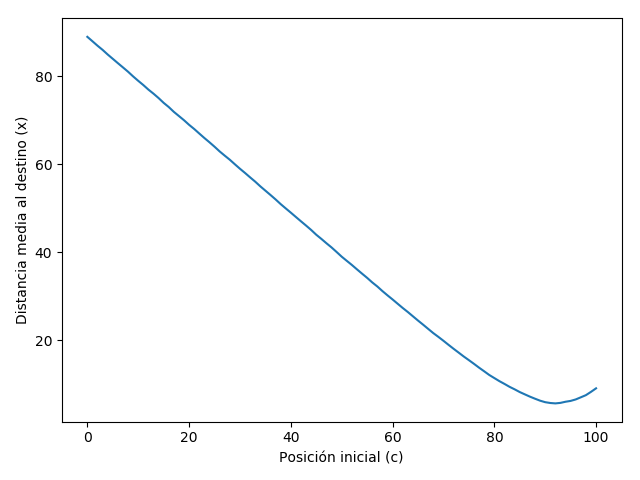
\includegraphics[scale=0.4]{img/x-100-10-90.png}
	\end{minipage}
	\begin{minipage}{0.5\textwidth}
	  \centering
	  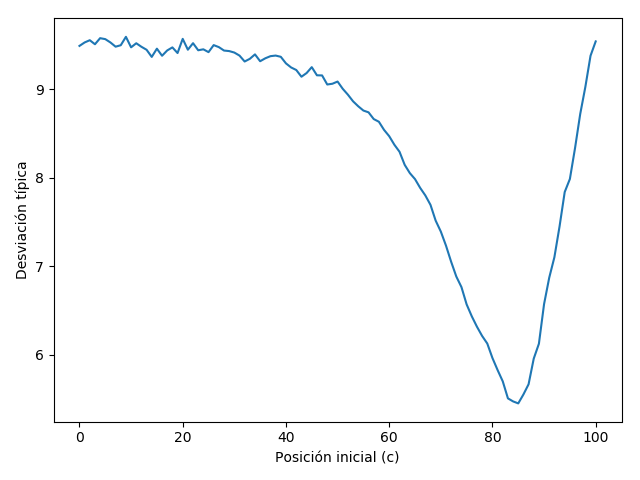
\includegraphics[scale=0.4]{img/dt-100-10-90.png}
	\end{minipage}
	\caption{Valores medios de las distancias y las desviaciones típicas con vision=10}
\end{figure}

Podemos ver que las gráficas siguen la misma tendencia que las gráficas de la ejecución por defecto y las del apartado anterior,
lo cual nos dice que, aun cambiando este parámetro, cuanto más cerca empecemos a buscar aparcamiento, más se reducirá la distancia
hasta el destino.

Sin embargo, con las gráficas no se puede apreciar bien cuánto se llega a reducir esta distancia, algo que si
apreciamos con valores numéricos, asi que voy a realizar otra ejecución con un abanico de valores más amplio para este parámetro.

\newpage

A continuación, una tabla con el resultado de esta ejecución:

\begin{table}[H]
\centering
\begin{tabular}{c|cc}
\textbf{Visión} & \textbf{Mejor posición inicial} & \textbf{Mejor distancia} \\ \hline
\textbf{0}      & 94                              & 6.55275                  \\ \hline
\textbf{5}      & 94                              & 6.29162                  \\ \hline
\textbf{10}     & 92                              & 5.64137                  \\ \hline
\textbf{15}     & 89                              & 5.26576                  \\ \hline
\textbf{20}     & 86                              & 5.03522                  \\ \hline
\textbf{25}     & 83                              & 4.9281                   \\ \hline
\textbf{30}     & 82                              & 4.82683                  \\
\end{tabular}
\end{table}

Como podemos observar, la mejor posición inicial es cada vez más lejana al destino, no obstante, la mejor distancia media también
se está reduciendo. Esto se debe a que, contra más visión se tenga de los aparcamientos que tenemos delante, no necesitaremos avanzar
hasta posiciones cercanas a nuestro destino, porque ya sabremos si hay aparcamiento o no.

\subsection{Probabilidad de encontrar aparcamiento}

Este parámetro sería el único que tiene aleatoriedad, ya que en un problema de la vida real, podemos saber dónde está nuestro destino
o el número de aparcamientos que somos capaces de ver, pero nunca tendremos control sobre la cantidad de aparcamiento libres que hay
en una calle.

Por esta razón, este parámetro será el que más merezca la pena estudiar. Vamos a comenzar sacando una tabla similar a la del apartado
anterior, ya que se pueden ver con más detalle los valores obtenidos en la ejecución.

\begin{table}[H]
\centering
\begin{tabular}{c|cc}
\textbf{\% de ocupación} & \textbf{Mejor posición inicial} & \textbf{Mejor distancia} \\ \hline
\textbf{25}     		 & 99                              & 0.273390                 \\ \hline
\textbf{50}     		 & 99                              & 0.743700                 \\ \hline
\textbf{75}     		 & 98                              & 2.162840                 \\ \hline
\textbf{80}     		 & 97                              & 2.955510                 \\ \hline
\textbf{85}     		 & 96                              & 4.138430                 \\ \hline
\textbf{90}     		 & 94                              & 6.494790                 \\ \hline
\textbf{95}     		 & 87                              & 13.458690                \\
\end{tabular}
\end{table}

Como podemos observar en la tabla, cuanto más bajo es el porcentaje de ocupación, más fácil es encontrar aparcamiento, y por tanto,
la distancia media a la que aparcamos es también muy baja. A medida que vamos aumentando este porcentaje, vemos como la posicion
inicial a la que se empieza a buscar aparcamiento está más lejos y, en cosecuencia, la mejor distancia aumenta.

Por último, vamos a mostrar una gráfica que muestra tres porcentajes de ocupación distintos para observar cómo cambia la distancia
entre ellos.

\begin{figure}[H]
\centering
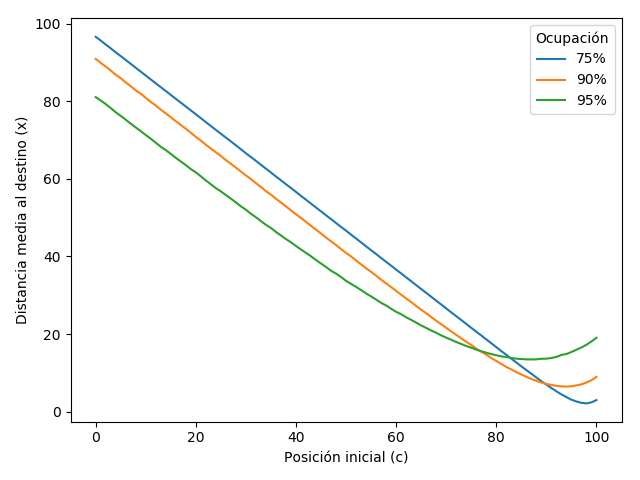
\includegraphics[scale=0.6]{img/x-100-2-75.png}
\caption{Valores medios de la distancias con distintos porcentajes de ocupación}
\end{figure}

\begin{figure}[H]
\centering
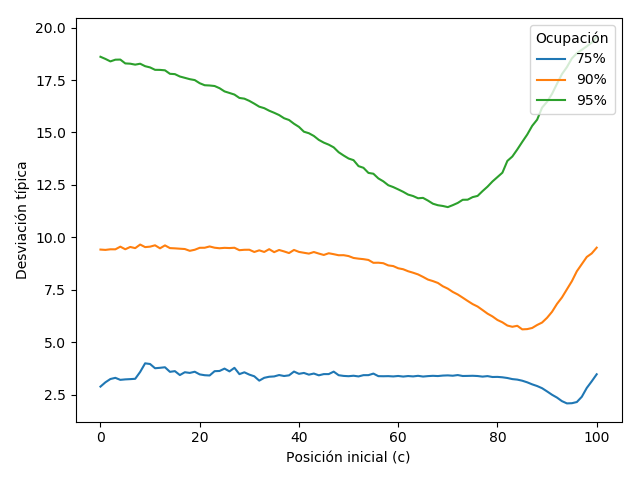
\includegraphics[scale=0.6]{img/dt-100-2-75.png}
\caption{Valores de la desviación típica con distintos porcentajes de ocupación}
\end{figure}

En la primera gráfica vemos cómo para un porcentaje bajo de ocupación, los valores de la gráfica llegan a sus mínimos cuando
se aproximan a $c=100$, porque da igual lo tarde que empiece a buscar un aparcamiento si las probabilidades de que encuentre
uno libre son bastante altas. Por otra parte, con un porcentaje de ocupación más alto, la distancia que tiene que recorrer
no es tan baja como antes, ya que si la posición inicial es cercana al destino la probabilidad de que se pase es más alta.

Esto último lo podemos corroborar con la gráfica de las desviaciones típicas, en la cual vemos cómo para estos altos porcentajes
de ocupación, la línea es mucho más pronunciada y ocupa unos valores más altos en comparación a los bajos porcentajes de ocupación.
Es decir, que cuanta más ocupación exista, es más propenso a pasarse del destino y a que las distancias aumenten.


\section{Experimentación con varios parámetros y valores extremos}

En esta sección no vamos a analizar todas y cada una de las posibilidades que tenemos, ni lo vamos a hacer tan en profundidad
como lo hicimos anteriormente, ya que nos podríamos extender demasiado.

Lo primero a tener en cuenta es, que la posición de destino $x$ la vamos a mantener en todas las ejecuciones como 100, porque
como hemos visto, es un parámetro muy poco relevante para la simulación. Dicho esto, pasemos a comentar cómo vamos a proceder
en esta experimentación.

Los parámetros a tener en cuenta serán:
\begin{itemize}[label=\textbullet]
	\item \textbf{Visión.} Que lo variaremos entre 0 y 100 para probar todas las posibilidades hasta llegar a valores extremos
	como el 100 que nos permitan ver todos los aparcamientos
	\item \textbf{Porcentaje de ocupación.} Que irá desde el 50\% hasta un $\approx100\%$, ya que el máximo hace que obtengamos
	un error (lógicamente, si todos los aparcamiento están ocupados, el programa buscará uno libre hasta que se quede sin memoria).
\end{itemize}

\newpage

En la siguiente tabla podemos observar los resultados de combinar todos los parámetros:

\begin{table}[H]
\centering
\begin{tabular}{c|c|c|c}
\textbf{Visión} & \textbf{\% de ocupación} & \textbf{Mejor posición inicial} & \textbf{Mejor distancia} \\ \hline
\textbf{2}      & \textbf{50}              & 98                              & 0.747980                 \\ \hline
\textbf{10}     & \textbf{50}              & 94                              & 0.662560                 \\ \hline
\textbf{50}     & \textbf{50}              & 90                              & 0.662040                 \\ \hline
\textbf{100}    & \textbf{50}              & 40                              & 0.659470                 \\ \hline
\textbf{2}      & \textbf{75}              & 98                              & 2.155360                 \\ \hline
\textbf{10}     & \textbf{75}              & 94                              & 1.766020                 \\ \hline
\textbf{50}     & \textbf{75}              & 73                              & 1.701890                 \\ \hline
\textbf{100}    & \textbf{75}              & 56                              & 1.698420                 \\ \hline
\textbf{2}      & \textbf{90}              & 94                              & 6.527760                 \\ \hline
\textbf{10}     & \textbf{90}              & 91                              & 5.662930                 \\ \hline
\textbf{50}     & \textbf{90}              & 72                              & 4.743880                 \\ \hline
\textbf{100}    & \textbf{90}              & 36                              & 4.712600                 \\ \hline
\textbf{2}      & \textbf{99}              & 31                              & 68.768227                \\ \hline
\textbf{10}     & \textbf{99}              & 34                              & 68.632362                \\ \hline
\textbf{50}     & \textbf{99}              & 30                              & 67.091072                \\ \hline
\textbf{100}    & \textbf{99}              & 18                              & 60.555672                \\ \hline
\end{tabular}
\end{table}

Analizando los valores que hemos obtenido, podemos ver como, pese a que el número de posiciones que vemos '\textit{Visión}' reduce
ligeramente la distancia, a lo que realmente afecta es a la posición inicial a partir de la cual empezamos a buscar aparcamiento.
Esto se debe lógicamente a la capacidad que tenemos de ver los siguientes aparcamientos, y en el caso de valores extremos (como es
el caso de verlos todos $vision=100$) obtenemos los valores más bajos.

En cuanto al porcentaje de ocupación, sin duda es el parámetro que más influye en la distancia a la que aparcaremos de nuestro
destino, ya que la mejora que se puede llegar a conseguir entre un 50\% de ocupación y un 99\% de ella es de aproximadamente 68
posiciones; mientras que la máxima mejora que se consigue gracias a la visión, es de aproximadamente de 8 posiciones. Incluso si
nos fijamos en la última fila de la tabla (donde tenemos los dos parámetros con valores extremos), podemos ver cómo ni teniendo
toda la visión de la calle, conseguimos bajar a un valor considerable la distancia.



\chapter{Mi primer modelo de simulación discreto}

\section{Experimentación para el número de repuestos}

\section{Influencia en el rendimiento de los parámetros}

\newpage

\begin{thebibliography}{5}

\bibitem{nombre-referencia}
Texto referencia
\\\url{https://url.referencia.com}

\end{thebibliography}

\end{document}

